\documentclass[a4paper,12pt]{article}

\usepackage[utf8]{inputenc}
\usepackage[T1]{fontenc}
\usepackage[portuguese]{babel}

\usepackage{graphicx}
\usepackage{geometry}
\usepackage{hyperref}
\usepackage{longtable}
\usepackage{float}
\usepackage{caption}
\usepackage{fancyhdr}
\usepackage{xcolor}

\geometry{margin=2.5cm}

% Metadados do documento (preencher)
\newcommand{\DocVersion}{1.0}
\newcommand{\POSName}{SVDI POS}
\newcommand{\POSVersion}{1.2.162.230226.1557-dev} % exemplo (do rodapé)
\newcommand{\Environment}{Certificação / Testes}
\newcommand{\TPAModel}{<preencher>}
\newcommand{\TPAFirmware}{<preencher>}

\title{Manual de Certificação\\Funções Multibanco no POS}
\author{Luís Gomes}
\date{Fevereiro 2026}

% Cabeçalho/Rodapé
\pagestyle{fancy}
\fancyhf{}
\lhead{\POSName\ -- Manual Certificação}
\rhead{Doc v\DocVersion}
\lfoot{POS v\POSVersion\ -- \Environment}
\rfoot{\thepage}

\begin{document}

\maketitle
\tableofcontents
\newpage
% -------------------------------------------------

\section{Âmbito e Objetivo}
Este documento descreve os fluxos funcionais das operações Multibanco no POS,
para efeitos de certificação, incluindo Venda, Devolução e Funções Supervisor.
As evidências apresentadas consistem em capturas de ecrã do POS durante execução
dos fluxos descritos.

\section{Ambiente de Certificação}
\begin{itemize}
  \item Produto: \POSName
  \item Versão do POS: \POSVersion
  \item Ambiente: \Environment
  \item Modelo do TPA: \TPAModel
  \item Firmware do TPA: \TPAFirmware
  \item Tipo de comunicação: <preencher>
\end{itemize}

% -------------------------------------------------
\section{Acesso ao POS}

\subsection{Página Inicial}

Após iniciar a aplicação, é apresentado o ecrã inicial do POS, com as opções de
acesso para o operador.

\begin{figure}[H]
    \centering
    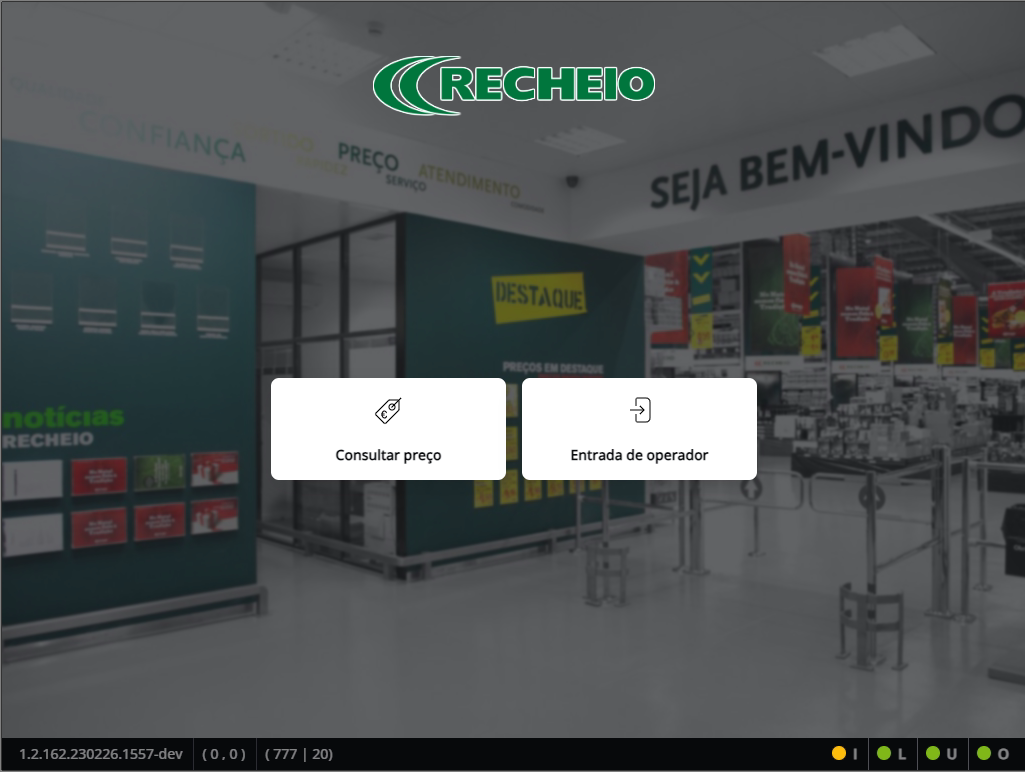
\includegraphics[width=0.85\textwidth]{images/pos_ecran_inicial.png}
    \caption{Página inicial do POS}
    \label{fig:pos-ecran-inicial}
\end{figure}

\subsection{Login de Operador}

Ao selecionar a opção \textbf{Entrada de Operador} no ecrã inicial, o POS apresenta
a página de login para autenticação do operador.

\begin{figure}[H]
    \centering
    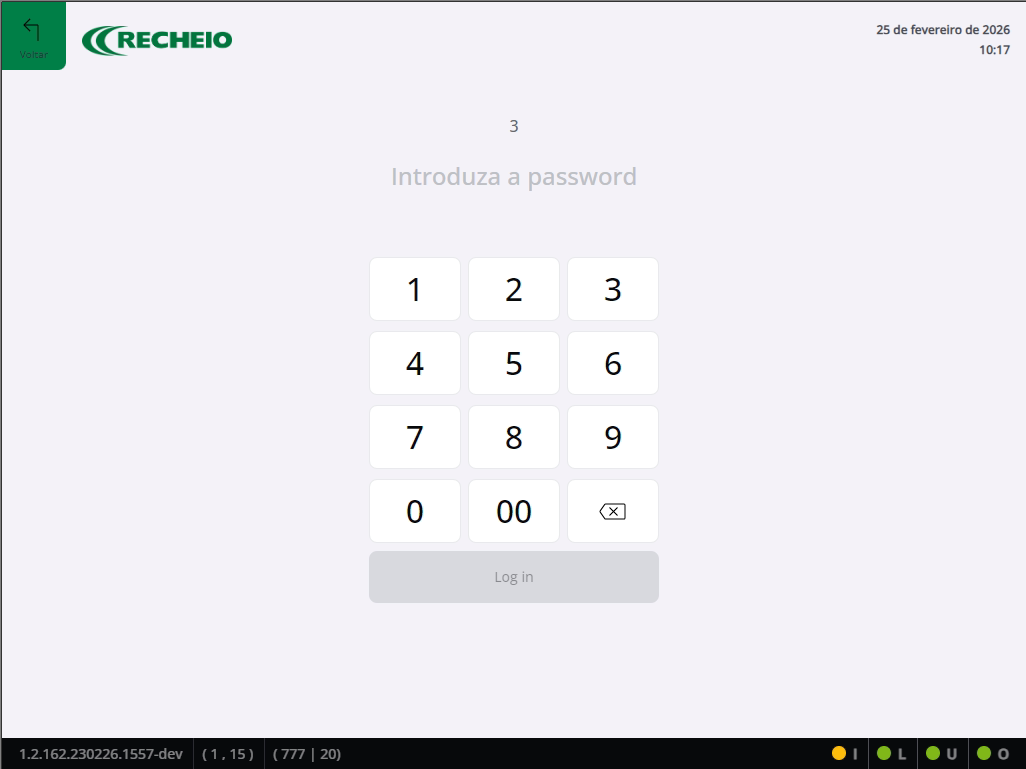
\includegraphics[width=0.85\textwidth]{images/login_operador.png}
    \caption{Página de login após selecionar \textbf{Entrada de Operador}}
    \label{fig:login-operador}
\end{figure}

\subsection{Identificação de Cliente}

Após o login efetuado com sucesso, o POS navega automaticamente para a página
de identificação do cliente.

\begin{figure}[H]
    \centering
    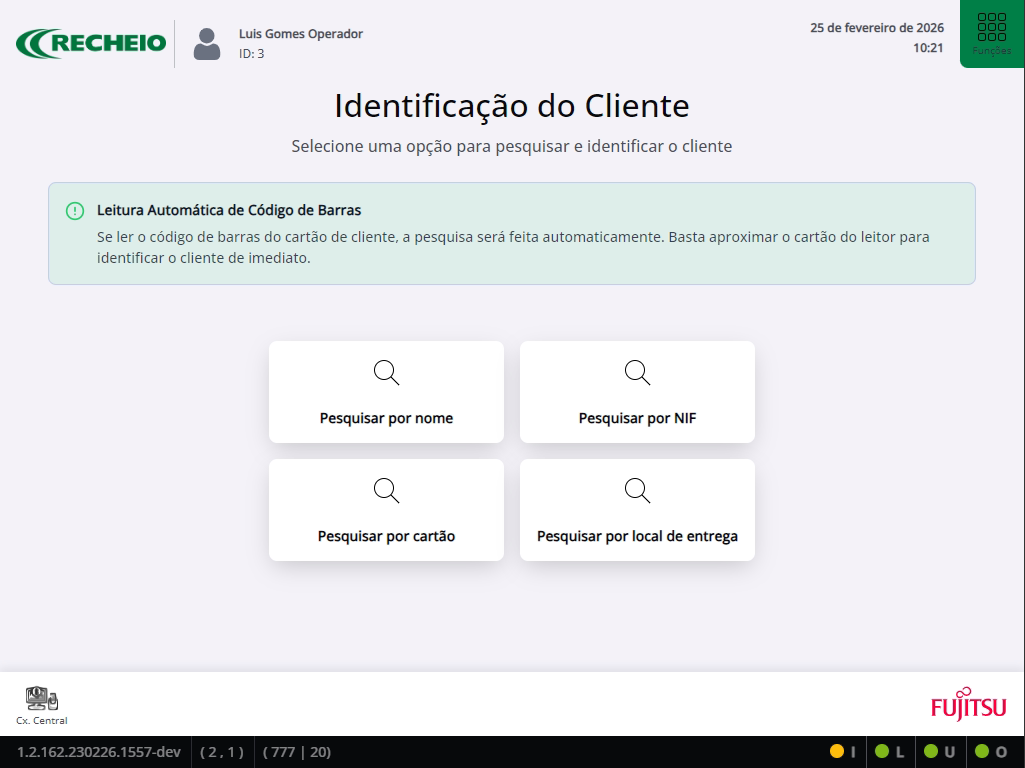
\includegraphics[width=0.85\textwidth]{images/identificacao_cliente.png}
    \caption{Página de identificação do cliente após login do operador}
    \label{fig:identificacao-cliente}
\end{figure}

% -------------------------------------------------
\section{Venda Multibanco}

\subsection{Descrição}

A operação de venda permite efetuar um pagamento através do terminal Multibanco,
com envio automático do montante a partir do POS.

\subsection{Pré-condições}

\begin{itemize}
    \item POS iniciado
    \item Sessão aberta
    \item Terminal operacional
\end{itemize}

\subsection{Fluxo da Operação}

\subsubsection{Passo 1 – Seleção da forma de pagamento}

O operador seleciona a opção Multibanco como forma de pagamento.

\begin{figure}[H]
    \centering
    \includegraphics[width=0.85\textwidth]{images/venda_passo1.png}
    \caption{Seleção da forma de pagamento}
    \label{fig:venda-passo1}
\end{figure}

\subsubsection{Passo 2 – Envio do valor ao terminal}

O POS envia automaticamente o montante ao terminal.

\begin{figure}[H]
    \centering
    \includegraphics[width=0.85\textwidth]{images/venda_passo2.png}
    \caption{Envio do valor ao terminal}
    \label{fig:venda-passo1}
\end{figure}

\subsubsection{Passo 3 – Confirmação da transação}

Após confirmação no terminal, o POS recebe a resposta da transação.

\begin{figure}[H]
    \centering
    \includegraphics[width=0.85\textwidth]{images/venda_passo3.png}
    \caption{Confirmação da transação}
    \label{fig:venda-passo1}
\end{figure}

\subsection{Resultado Esperado}

\begin{itemize}
    \item Transação aprovada
    \item Registo da operação no POS
    \item Impressão do talão (se aplicável)
\end{itemize}

% -------------------------------------------------
\section{Devolução Multibanco}

\subsection{Descrição}

A operação de devolução permite reembolsar uma transação previamente efetuada.

% Adicionar fluxo semelhante ao da venda

% -------------------------------------------------
\section{Funções Supervisor}

\subsection{Consulta de Totais}

Descrição da função.

\subsection{Fecho de Lote}

Descrição da função.

\subsection{Reimpressão}

Descrição da função.

% -------------------------------------------------
\section{Tratamento de Erros}

\begin{longtable}{|p{3cm}|p{5cm}|p{5cm}|}
\hline
Código & Descrição & Comportamento do POS \\
\hline
 & & \\
\hline
\end{longtable}

\end{document}
